\chapter{Evaluation und Demonstration}
In diesem Kapitel sollen die Ergebnisse des im Rahmen der Arbeit entwickelten Prototypen, anhand der zuvor definierten Anforderungen und Lösungen, bewertet und vorgestellt werden.
Im Anschluss daran wird eine Demonstration des Systems durchgeführt.

\section{Evaluation des Systems}
\label{evaluation-des-system}
Der Prototyp von CloudGrid wurde ausschließlich auf einem Linux Mint System getestet und ist dort voll lauffähig.
Linux Mint basiert auf Ubuntu, sodass die zwei meistgenutzten Linux Distributionen\footnote{\url{http://distrowatch.com/dwres.php?resource=popularity}} unterstützt werden.
Sowohl Windows als auch Mac OS wurden bei der Entwicklung des Prototypen nicht getestet.

Um die GUI korrekt darstellen zu können, werden Browser benötigt, welche HTML5 und CSS3 unterstützen.
Dazu zählen Google Chrome, Firefox, Safari und auch Opera, sowie die Internet Explorer ab Version 10.
Es kann bei unterschiedlichen Browsern kleinere Abweichungen bei der Positionierung von Elementen geben, welche sich jedoch nicht auf die Funktionalität der GUI auswirken.
Dieses Verhalten resultiert aus der unterschiedlichen Interpretation von \ac{HTML} und \ac{CSS} der einzelnen Browser.

Ein weiterer Schwerpunkt liegt in der Integration weiterer Cloudservices in CloudGrid.
Wenn ein Dienst zur Anwendung hinzugefügt werden soll, müssen dazu drei Anpassungen vorgenommen werden.
In den Ordner \frqq provider\flqq\ muss zuerst eine Klasse integriert werden, welche, entsprechend der Klassen der bestehenden Anbieter, die Funktionalitäten der Clouddienste abbildet.
Daraufhin muss der einzubindende Anbieter in der Konfigurationsdatei \frqq provider.json\flqq\ im Ordner \frqq models\flqq\ aufgenommen werden.
In dieser Datei werden alle Parameter, die bei der Authentifizierung mittels OAuth benötigt werden, hinterlegt.
Um abschließend den Anbieter auch in der \ac{GUI} verfügbar zu machen, muss ein Button in der View \frqq connect.html\flqq\ hinterlegt werden, so wie die entsprechende Controllerlogik in der \frqq connect.js\flqq .
Die Auswahl der Cloudservices beim Upload wird daraufhin automatisch von CloudGrid durchgeführt.
Der gesamte Vorgang sollte, in einer späteren Version von CloudGrid, noch modularer und generischer gestaltet werden, sodass ein Entwickler leichter weitere Anbieter integrieren kann.

Weiterhin erweist sich die im Systementwurf getätigte Annahme, dass der Dateiupload, weitaus langsamer ist, als die Dateioperationen als richtig.
Bei einem Test mit einer 50 \ac{MB} großen Datei und lediglich einem Cloudservice, dauerten die Dateioperationen im Durchschnitt 7 Sekunden, wohingegen der Upload der Teilstücke im Durchschnitt rund 2 Minuten dauerte.
Diese Werte wurden auf einem Laptop mit einem Intel Core i3 mit 2,4 \ac{GHz}, 3 \ac{GB} Arbeitsspeicher, sowie einer Festplatte mit einem \ac{SATA} Anschluss und 7200 \ac{upm} ermittelt.
Die Uploadgeschwindigkeit wird laut Internetprovider mit 10 mbit/s angegeben.
Dieser Engpass kann leider nicht umgangen werden.
Vor dem Upload der Teilstücke einer Datei, werden diese bereits komprimiert, um den Vorgang zu beschleunigen.
Jedoch reicht das nicht aus, um das Verhältnis auszugleichen.
Dateioperationen werden zum jetzigen Stand der Technik schneller durchgeführt, als das Verschicken von Daten über ein Netzwerk oder das Internet.
Lediglich durch die Implementierung der, bereits im Abschnitt \ref{implementierung-realisierung-anwendungslogik} erwähnten fehlenden Unterstützung der Events \frqq Verschieben\flqq\ und \frqq Umbenennen\flqq\ bei der Ordnerüberwachung, können unnötige Uploadvorgänge vermieden werden, was Ressourcen einsparen würde.
Jedoch bleibt auch dadurch die Grundproblematik bestehen.

\section{Demonstration des Systems}

Um die Anwendung zu starten muss die Linux Konsole geöffnet werden und in den entsprechenden Ordner von CloudGrid navigiert werden.
Dort muss entweder der Befehl \frqq node CloudGrid.js\flqq\ oder alternativ die Makefile mittels \frqq make start\flqq\ ausgeführt werden.
Daraufhin ist die \ac{GUI} im Browser unter \url{http://localhost:8080} oder alternativ unter \url{http://cloudgrid.local:8080} erreichbar.
Beim ersten Start der Anwendung bekommt der Benutzer eine Einstellungsseite angezeigt, welche in Abbildung \ref{fig-demo-first-start} zu sehen ist.

\begin{figure}[H]
  \centering
  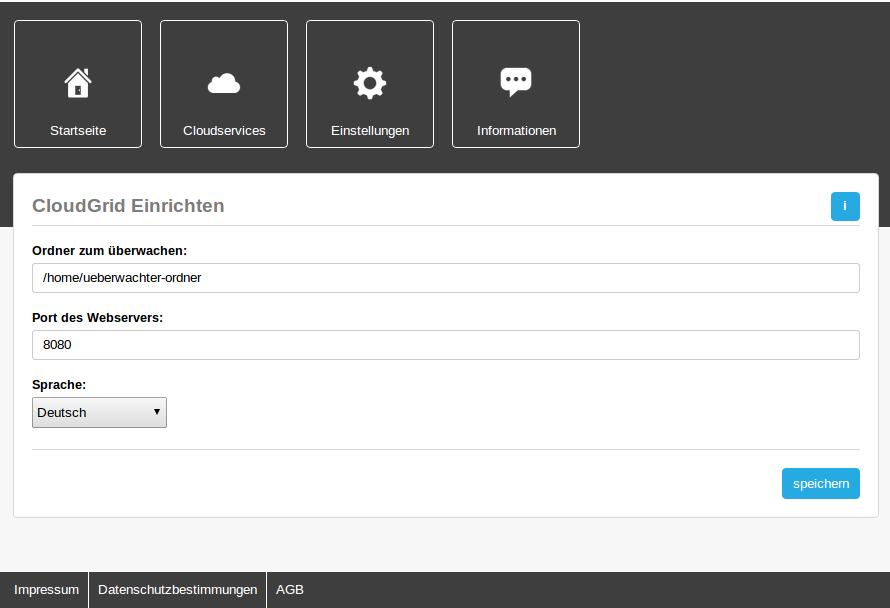
\includegraphics[scale=0.4]{resources/Bilder_Kapitel_6/first-start.png}
  \caption{Einstellungsseite beim ersten Start der Anwendung}
  \label{fig-demo-first-start}
\end{figure}

Hier kann der Benutzer den zu überwachenden Ordner, den Port auf dem der Webserver laufen soll und die Sprache einstellen.
Dabei sind alle Werte vordefiniert, sodass der Nutzer sich leichter in diese Seite einfinden kann.
Durch Anklicken des blauen \frqq i\flqq\ Buttons in der rechten oberen Ecke erhält er darüber hinaus Informationen zur Seite.
Wenn er die Einstellungen gespeichert hat, wird eine Erfolgsseite angezeigt.
Sollte er Felder nicht ausfüllen, erscheint eine entsprechend Fehlermeldung und die Felder können nochmals bearbeitet werden.

Sobald die Speicherung erfolgreich war, muss sich der Benutzer im Menüpunkt \frqq Cloudservices\flqq\ mit den einzelnen Diensten verbinden.
Abbildung \ref{fig-demo-cloudservices} zeigt diese Seite auf.
Der Benutzer muss zuvor seine \frqq client id\frqq , seinen \frqq client secret\flqq\ und die \frqq redirect uri\flqq\ in den entsprechenden Formularfelder hinterlegen, um daraufhin durch einen Klick auf das entsprechende Logo des Anbieters, die Authentifizierung durchzuführen.
Er wird daraufhin zum Anbieter weitergeleitet, wo er sich Einloggen muss, um dann CloudGrid die Berechtigung zu geben, auf seine Benutzerdaten zuzugreifen.
Abschließend wird er wieder zur Cloudservicesseite zurückgeleitet und erhält einen Hinweis, über die erfolgreiche Verknüpfung mit dem Service.
Dienste welche bereits erfolgreich verbunden sind, erhalten einen grünen Haken am Logo, nicht verbundene Dienste ein rotes Kreuz.

\begin{figure}[H]
  \centering
  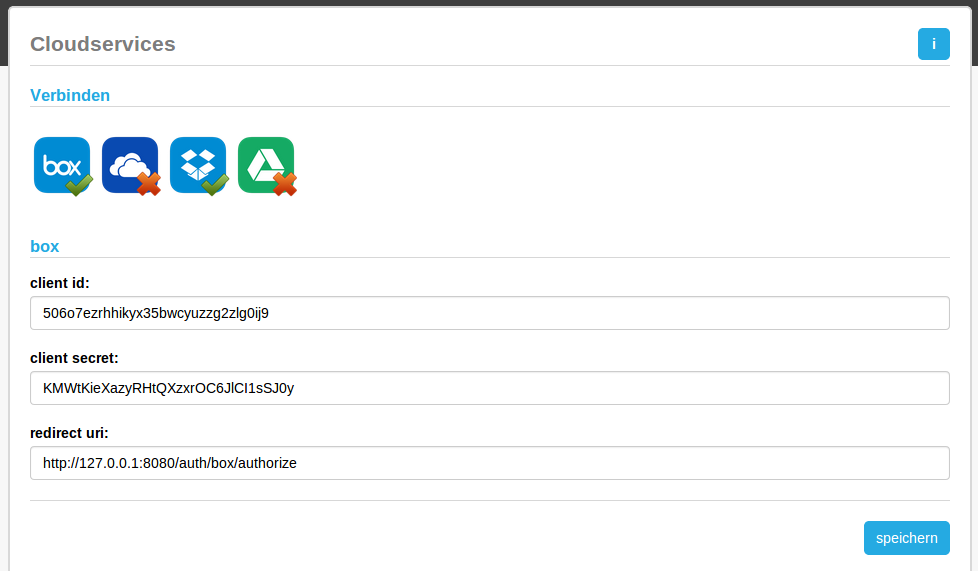
\includegraphics[scale=0.4]{resources/Bilder_Kapitel_6/cloudservices.png}
  \caption{Seite zum Verbinden und Bearbeiten der Cloudservices}
  \label{fig-demo-cloudservices}
\end{figure}

Wenn auch dieser Vorgang abgeschlossen ist, kann der Benutzer Ordnerüberwachung zum ersten mal starten.
Im Header der \ac{GUI} befindet sich ein Button, welcher betätigt werden muss.
Initial ist die Ordnerüberwachung deaktiviert.
Abbildung \ref{fig-demo-watchr-not-started} zeigt den Informationstext und den Button auf.

\begin{figure}[H]
  \centering
  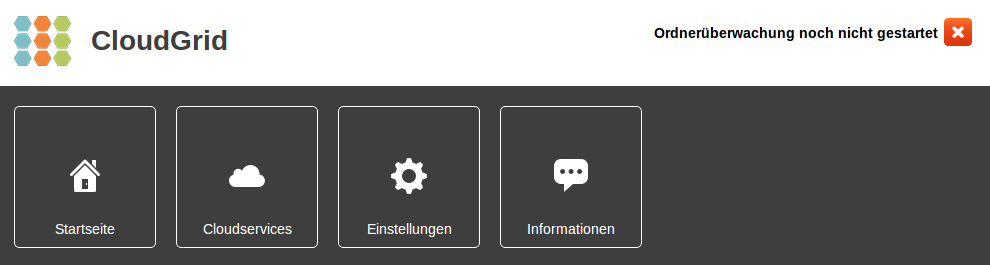
\includegraphics[scale=0.4]{resources/Bilder_Kapitel_6/watchr_not_started.png}
  \caption{Die Ordnerüberwachung ist deaktiviert}
  \label{fig-demo-watchr-not-started}
\end{figure}

Sobald der Benutzer den Button anklickt, wird eine Warteanimation gestartet.
Wenn der Vorgang abgeschlossen ist, bekommt er die Information, welche in Abbildung \ref{fig-demo-watchr-started} dargestellt ist, angezeigt.

\begin{figure}[H]
  \centering
  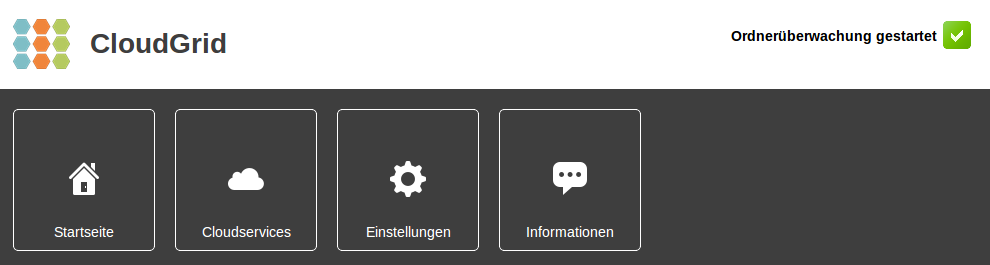
\includegraphics[scale=0.4]{resources/Bilder_Kapitel_6/watchr_started.png}
  \caption{Die Ordnerüberwachung wurde gestartet}
  \label{fig-demo-watchr-started}
\end{figure}

Die Ordnerüberwachung ist somit gestartet und jegliche Veränderungen werden erkannt.
Alle Dateien, welche sich in dem zu überwachenden Ordner befinden, werden zudem beim Start initial eingelesen und zu den Clouddiensten geuploaded.
Der Benutzer hat jederzeit die Möglichkeit, die Ordnerüberwachung an- und abzustellen.
Dieses Verhalten kann gewünscht sein, wenn beispielsweise größere Veränderungen in dem Ordner durchgeführt werden oder die gesamte Bandbreite der Internetverbindung benötigt wird.

Jegliche Vorgänge kann der Benutzer dabei im Menüpunkt \frqq Informationen\flqq\ einsehen und den Fortschritt verfolgen.
Abbildung \ref{fig-demo-logging} zeigt beispielhaft diese Seite auf.
Die Einträge in dem Textfeld werden im zwei Sekundentakt aktualisiert, sodass der Benutzer die Seite nicht manuell aktualisieren muss.
Zudem kann er sich ältere Einträge mittels der Datumsauswahl oberhalb des Informationsfensters anzeigen lassen.

\begin{figure}[H]
  \centering
  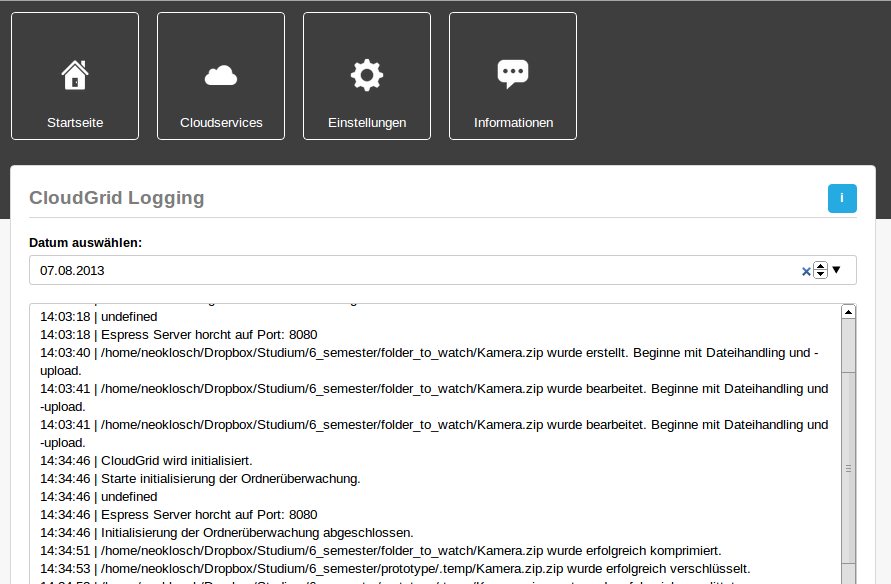
\includegraphics[scale=0.4]{resources/Bilder_Kapitel_6/logging.png}
  \caption{Informationsseite von CloudGrid}
  \label{fig-demo-logging}
\end{figure}

Die Seite \frqq Einstellungen\flqq\ ähnelt der Seite, die der Benutzer beim ersten Start der Anwendung angezeigt bekommt.
Jedoch sind hier weniger Einstellmöglichkeiten verfügbar.
Im Prototypen ist es nicht möglich, den zu überprüfenden Ordner zu wechseln.
Das Problem liegt in einer erhöhten Komplexität des Dateihandlings.
Es muss geklärt werden, was mit den Dateien im bestehenden Ordner passiert.
Dabei können zwei Ansätze verfolgt werden.
Im ersten Fall werden alle Dateien in den neu zu überwachenden Ordner kopiert und verbleiben bei den Clouddiensten.
Der zweite Fall belässt alle Dateien im ursprünglichen Ordner und löscht die entsprechenden Teilstücke bei den Clouddiensten.
Beide Verfahren haben ihre Vor- und Nachteile.
Im Prototypen wurde daher lediglich das einmalige Auswählen des Ordner integriert.
Jedoch können wie bereits zuvor, sowohl die Sprache, als auch der Port des Webservers bearbeitet werden.

Im Footer der Seite wurden hingegen die drei Seiten \frqq Impressum\flqq , \frqq AGB\flqq\ und \frqq Datenschutz\flqq\ aufgenommen.
Da diese funktional nicht relevant sind, sind sie momentan mit Blindtext gefüllt, bedingt durch die im Abschnitt \ref{systementwurf-recht} erwähnte Problematik, dass diese inhaltlich durch einen Anwalt erstellt werden müssen.

Letztendlich wurde das in Abschnitt \ref{systementwurf-praesentation} angedachte Designkonzept komplett umgesetzt und erfüllt funktional alle Anforderungen.
Auf allen Seiten ist ein einheitliches Layout zu erkennen, welches mit der \frqq hogan\flqq\ Templateengine modular umgesetzt wurde.
